\chapter{実装}
\label{chap:implementation}

本章では,第2章で述べたシステムの設計を受け,Gyaonの実装について述べる.

\newpage

\section{システム構成}
Gyaonは,ユーザが実際に録音/再生するためのクライアントアプリケーションと,
アップロードされた音声を保存/管理するサーバから構成される.構成図を図\ref{system}に示す.

\begin{figure}[H]
\centering
\fbox{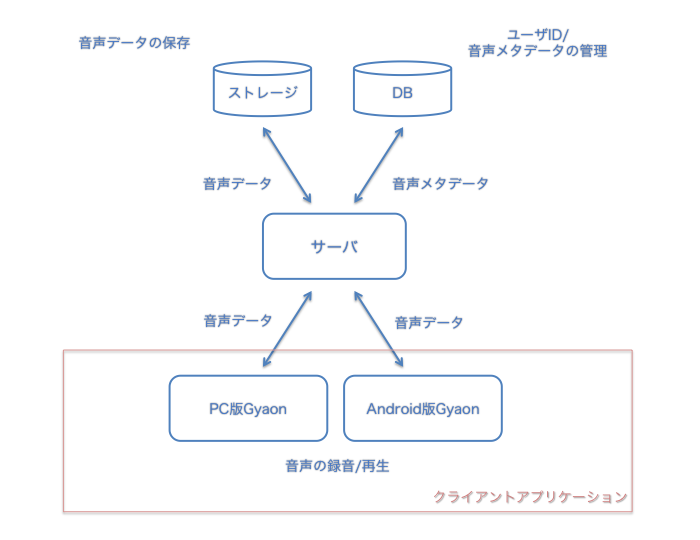
\includegraphics[width=15cm]{images/system.png}}
\caption{Gyaonシステムの構成図}
\label{system}
\end{figure}

\section{サーバ}
サーバはNode.js\footnote{\textsf{https://nodejs.org}}
とそのWebアプリケーションフレームワークであるExpress\footnote{\textsf{http://expressjs.com/ja/}}
によって実装されている.音声データの保存をAmazon S3
\footnote{\textsf{Amazon Web Servicesによって提供されるオンラインストレージサービス.https://aws.amazon.com/jp/s3/}},
DB管理をmLab\footnote{\textsf{MongoDBベースのクラウドDBサービス.https://mlab.com/}}にて行っている.

\subsection{DBスキーマ}

DBでは以下のようなスキーマを定義し,音声データを管理している.

\vspace{4mm}
\begin{lstlisting}
var soundSchema = mongoose.Schema({
    lastmodified: Date,     /* 録音時刻 */
    user: String,           /* ユーザID */
    name: String,           /* ファイル名 */
    key: String,            /* S3key */
    size: Number,           /* ファイルサイズ */
    time: Number,           /* 再生時間 */
    comment: String,        /* コメント */
    location_x: Number,     /* 位置情報 */
    location_y: Number
})
\end{lstlisting}

\section{PC版クライアント}
PC版クライアントはHTML/CSS/JavaScriptで実装されており,ブラウザ上のWebアプリケーションとして動作する.
%各機能の実装について述べる.
%特筆すべき実装
%詳細な実装

\subsection{WebAudioAPI}
%WebAudioAPIを解説する
録音/再生といった主要な音声機能は,
HTML5 audio\footnote{\textsf{https://www.w3.org/TR/html5/embedded-content-0.html\#the-audio-element}}
並びにWebAudioAPI\footnote{\textsf{https://www.w3.org/TR/webaudio/}}によって実装されている.

HTML5 audioはHTMLドキュメント内に音声を埋め込むことができ,以下のようなAudio要素を宣言することで利用できる.

\vspace{4mm}
\begin{lstlisting}
<audio src="/test/audio.mp3"></audio>
\end{lstlisting}

WebAudioAPIは高度な音声処理や音声合成を行えるJavaScriptAPIであり,
Audio要素を操作したり,エフェクトを加えることができる.

\subsection{音声リストの同期}
複数のユーザが同じユーザIDを使用していても,音声リストはリアルタイムに同期される.
これはNode.jsのWebSocketライブラリ「Socket.IO\footnote{\textsf{http://socket.io}}」によって実装されており,
サーバに音声がアップロードされると,音声リストの更新情報がブラウザに通知される.

%\subsection{プリレコーディング機能}
%shift/pushしている部分のコードを貼る

%録音ボタンを押す前からの音声を撮れる
%音声を入れてる配列の操作で
%〜は,以下のように実装されている
%プリレコーディング機能は,
%音声データを格納する配列へのshift/push
%配列を
%ことで実現されている.
%
%\vspace{4mm}
%\begin{lstlisting}
%preRecScriptProcessor.onaudioprocess = (event) => {
%    const channel = event.inputBuffer.getChannelData(0)
%    if(preRecAudioBufferArray.length * BUFFER_SIZE > SAMPLE_RATE * PREREC_SEC) {
%        preRecAudioBufferArray.shift()
%    }
%    preRecAudioBufferArray.push(new Float32Array(channel))
%}
%\end{lstlisting}

\subsection{Gyaonキー}
%Karabinerを使っている
%録音するシェルスクリプトを叩かせている
%スクリプト本体やkarabiner設定ファイルを貼る

Gyaonキーは,キーボードをカスタマイズするMacアプリケーション
「Karabiner\footnote{\textsf{https://pqrs.org/osx/karabiner/index.html.ja}}」
を利用して実装されている.
Karabinerを利用すると,キーボードが出力する文字列をカスタマイズしたり,
任意のキーでアプリを起動するよう指定できる.

筆者の環境では,command + fn キーで録音/アップロードを行うシェルスクリプトを実行するよう設定している.
以下にKarabiner設定ファイル(XML)の一部を示す.

\vspace{4mm}
\begin{lstlisting}
<vkopenurldef>
  <name>KeyCode::VK_OPEN_URL_SHELL_GYAON_START</name>
  <url type="shell">
    <![CDATA[    /bin/sh $HOME/.gyaon/start.sh    ]]>
  </url>
</vkopenurldef>
<item>
  <name>CMD_R + FN -> GYAON</name>
  <identifier>gyaon</identifier>
  <autogen>
    __SimultaneousKeyPresses__
    KeyCode::COMMAND_R, KeyCode::FN,
    KeyCode::VK_OPEN_URL_SHELL_GYAON_START,
    Option::NOREPEAT,
    Option::KEYTOKEY_AFTER_KEYUP,
    KeyCode::VK_OPEN_URL_SHELL_GYAON_STOP,
  </autogen>
</item>
\end{lstlisting}


\section{Android版クライアント}
Android版クライアントはJavaで実装されており,通常のAndroidアプリケーションとして動作する.
常駐型の録音ボタンは,バックグラウンド実行が可能なServiceとして実装されている.

%現状serviceを使っている
%常駐ボタンが邪魔だったりするので,他の方法を考えたい
%スマホを起動しなくてもいい方法
%    専用ボタンとか
%    ヘッドセットとか
